\documentclass[
10pt, % Main document font size
a4paper, % Paper type, use 'letterpaper' for US Letter paper
oneside, % One page layout (no page indentation)
%twoside, % Two page layout (page indentation for binding and different headers)
fleqn,
leqno,
headinclude,footinclude, % Extra spacing for the header and footer
BCOR5mm, % Binding correction
]{scrartcl}

\usepackage{memoco}
\title{\normalfont{Methods and Models for Combinatorial Optimization \\
                   Report}}

\subtitle{University of Padua}

\author{Sebastiano Valle}

\date{\today}
 % define header elements



\begin{document}

\maketitle
\setcounter{tocdepth}{3}
\setcounter{secnumdepth}{0}
\tableofcontents

\newpage
\section{Introduction}
The purpose of this document is to describe how a particular combinatorial
optimization problem was solved by adopting several approaches in order to
obtaining a value for the objective function in a limited amount of time without
losing too much quality in the goodness of the solution.

\subsection{(Brief) Problem description}
The assignment is an instance of the classical \textit{Travelling Salesman
Problem}: a company has to drill holes on a board, so that electrical components
can be placed over the board by inserting their pins into the holes. The goal
that the company is trying to achieve is to minimize the time the drill
takes to make all the holes\footnote{as well as the distance that the drill
covers by moving}.

I will refer to this problem as the \textbf{drilling problem} from now on.

\paragraph{Assumptions}
\begin{itemize}
  \item the starting point can be arbitrarily chosen;
  \item the time that is needed to move from a node $i$ to a node $j$ depends
    \textit{only} on the distance \dist{i}{j}.
\end{itemize}

\subsection{How to run the program}

In Section \ref{sec:instructions} there are some basic hints and references
to use both the Part I and Part II of the assignment.

Please refer to that section to use the program correctly.

\newpage\section{Part I -- Exact method}

In this section I'll describe the implementation details for the first part of
the exercise, e.g. the one that finds the global optimum thanks to \cplex.

\subsection{Data structures}
Before calling the proper API to solve the optimization problem, the main
procedure of the program has to write down the problem in the \cplex{}
environment.

This goal is indeed accomplished by calling a sub-procedure \texttt{setupLP}
that is accountable for generating variables and constraints: thus, along this
function we need to keep track of the indexes of the variables we declared so
that we are able to refer to them when creating the constraints.

An initial solution may be to inspect how variables are defined and then
re-compute their indexes each time we need to refer to a given variable.

It is easy to see that this approach may lead to poor code quality: if variables
were generated in another procedure and then the incomplete problem was handed
off to another programmer, it would have to look at \textit{how} her colleague
defined the variables (all of this without guarantees that the variables
generation is fixed).

Thus, an (pretty straightforward) alternative solution is to store variables'
indexes in a ``map'' while generating the variables, i.e. an $n$-dimensional
vector where $n$ is the dimension of a certain variable\footnote{if a variable
$x_{i,j}$ is indexed with two factors $i$ and $j$, then the map relative to
$x_{i,j}$ will have two dimensions}.
Therefore, variables and constraints generation are now loosely coupled, which
is clearly a good software engineering discipline: in fact, in the previous
scenario the former programmer will pass the indexes maps to the latter, without
requiring her to know any implementation detail.

\subsection{Variables generation}
In \cplex, before you create the constraints you (reasonably) have to declare
the variables you are going to use. Since in this situation the model is
relatively small, it is (arguably) more important to create it in a more
expressive and clear manner rather than it is to make it efficiently.

For this reason, variables of the sort $x_{i,j}$ and $y_{i,j}$ were defined in
two separated cycles, iterating twice over the range of all $i,j\in{N}$, where
$N$ is the set of holes.

\subsection{Constraints generation}
As it was done for variables, clarity has been chosen over efficiency for
constraints too. Thus, constraints were added in several blocks so anyone can
be able to understand what the program is doing at that line of code by looking
at the comments at the beginning of each block.

\subsection{Sample data generation}

\newpage\section{Part II}

In this section I'll describe the implementation details for the second part of
the exercise, that is the one that tries to find a good solution thanks to a
meta-heuristic.

For this task I chose to use a classical genetic algorithm in which:

\begin{itemize}
	\item the stopping criterion is a time-out;
	\item solutions are encoded as in the first part, i.e. ordered sequence of
		visited nodes;
	\item the initial population is obtained by creating some solutions with true
		randomness and the other with a simulated annealing limited by the number
		of iterations;
	\item solutions are chosen from the population by using linear ranking;
	\item recombination is performed by both an order crossover and a mutation;
	\item solutions are evaluated by computing the value of the objective
		function for each one of them;
	\item elements of the population are replaced by using elitism, i.e. keeping
		the best ones and picking at random among the rest the elements which will
		be replaced by offspring.
\end{itemize}

In order to make the code more maintainable, I isolated each functionality in
its own class, so that if we want to \textit{tune} the genetic algorithm we can
do it by changing a value related to a specific part of the program.

\subsection{Design decisions}

\paragraph{Simulated Annealing} By adopting the Simulated Annealing method, I
improved the initial population that before was created purely random.

I chose this particular technique due to two of its main advantages:
\begin{itemize}
	\item Simulated Annealing is a local search, thus I've been able to
		\textit{train} the initial population;
	\item Simulated Annealing does not always choose an improving neighbour, so
	  the program does not lose too much in diversification in the first steps.
\end{itemize}

\paragraph{Mutation} Many choices like elitism or linear ranking push the
program to evolve with intensification.

Mutation was not present in the first design of the algorithm. I introduced it
to overcome an unwanted pattern that I recognized after several runs: it
happened that one or two traits used to emerge against all the others. Thus, by employing these two techniques I've been able to introduce diversification
in the genetic algorithm and obtain more variability in the solutions.

In fact, the mutation I've implemented ignores completely the fitness of the
solution and adds it to the offspring. The mutation present in this genetic
algorithm consists of a 2-opt operation, that is a complete substring reversal
in the encoding of the solution.

\subsection{Parameter calibration} \label{sec:par-calib}

I tuned the program by varying the following parameters:

\begin{itemize}
	\item \textbf{time-out}, i.e. the stopping criterion ($5$ or $60$ seconds)
	\item \textbf{mutation probability}, i.e. the probability for a mutation to
		occur in a generation ($0.5$ or $1$)
	\item \textbf{number of elements of the initial population generated with
		heuristic} ($5$ or $0$)
	\item \textbf{elite size}, i.e. the elite group size ($3$ or $20$)
\end{itemize}

Obviously, I ran the genetic algorithm several times before doing the
comparison against the exact method of the part I. Therefore I was able to
calibrate the parameters listed above and find some values indicated within
brackets that looked significant to me\footnote{by saying this, I mean that
by choosing either one of the two values we would obtain a noticeable
difference in the goodness of the objective function}.






\newpage\section{Results for the Part I}

In this section I will show how the exact method performed under different
circumstances and describe each one of them.

\subsection{Scenarios}

I prepared different scenarios for the evaluation of the programs, which
correspond more or less to the different instances I provide as input with a
little of configuration.

Wrapping up, we have these different kinds of instances:

\begin{itemize}
  \item \textit{345}, i.e. the Pythagorean instance;
  \item \textit{tsp12} and \textit{tsp60}, i.e. the hard-coded instances
    provided by the professor;
  \item \textit{gerber}, i.e. an instance generated out of a Gerber file;
  \item \textit{ru}, i.e. instances generated with the Random Uniform method;s
  \item \textit{rg}, i.e. instances generated with the Random Grid Uniform
    method, in which I considered the euclidean distance between points
    ($\sqrt{(x_a - x_b)^2 + (y_a - y_b)^2}$);
  \item \textit{rg\_Manh}, i.e. instances generated with the Random Grid Uniform
    method, in which I considered the Manhattan distance between points
    ($|x_a - x_b| + |y_a - y_b|$).
\end{itemize}

While the first four instances were generated with a fixed number of
holes\footnote{I created only one Gerber instance, so I put \textit{gerber} in
the group of ``fixed'' instances}, the three random types of instances are
generated by means of some parameters:

\begin{itemize}
  \item the number of holes $n$;
  \item the size of the board $s$, which is not an absolute value but a size
    factor that, together with the number of holes, yields the actual size of
    the board\footnote{in this way, boards with different number of holes can
    be compared more reasonably};
  \item the number of divisions per side $d$ for the $rg^*$ instances, so that
    we divide the board into a grid of $d^2$ cells.
\end{itemize}

In particular, I set up the following configurations for the tests:

\begin{table}[H]
  \centering
  \begin{tabular}{|l|c|r|}
    \hline
    \textbf{\textit{h}} & \textbf{\textit{s}} & \textbf{\textit{d}} \\
    \hline
    \hline
    10 & 10  & 2 \\
    \hline
    10 & 100 & 2 \\
    \hline
    10 & 10  & 4 \\
    \hline
    10 & 100 & 4 \\
    \hline
    50 & 10  & 2 \\
    \hline
    50 & 100 & 2 \\
    \hline
    50 & 10  & 4 \\
    \hline
    50 & 100 & 4 \\
    \hline
  \end{tabular}
  \caption{Settings for tests}
  \label{tab:settings}
\end{table}

Thanks to these configurations, we range over different parameters of the
instances' creation.

\subsection{Part I performance}

Hereafter, I show how the exact method performed with each possible
configuration. For convenience, I'll group fixed-size instances together.


\newpage\section{Results for Part II}

In this section I will show:
\begin{itemize}
  \item how I decided to conduct tests for the part of the assignment related
    to meta-heuristic;
  \item some statistics, i.e. minimum, maximum, mean of the objective function.
\end{itemize}

\subsection{Scenarios}

As I did for the tests of the Part I, I prepared a bit of configuration also
to test the program that uses the genetic algorithm.

In fact, I automatized the tests to run by combining the settings shown in
\ref{sec:resI-scenarios} with the tuning I made for the algorithm (see
\ref{sec:par-calib}).

So, I tested all the scenarios (\textit{345}, \textit{tsp12}, \textit{tsp60},
\textit{gerber}, \textit{ru}, \textit{rg} and \textit{rg\_Manh}) with all the
configurations shown in Table \ref{tab:settings}, running the algorithm at
least seven times with each of the following calibrations\footnote{all the
tests were run with a population size of $55$}:

\begin{table}[H]
  \centering
  \begin{tabular}{|l|c|c|c|r|}
    \hline
    \textbf{\textit{name}} & \textbf{\textit{t}} (s) & \textbf{\textit{m}} &
    \textbf{\textit{h}} & \textbf{\textit{e}} \\
    \hline
    \hline
    Avg & $5.0$ & $50\%$ & 5 & 3 \\
    \hline
    BE & $5.0$ & $50\%$ & 5 & 20 \\
    \hline
    Mut & $5.0$ & $100\%$ & 5 & 3 \\
    \hline
    NH & $5.0$ & $50\%$ & 0 & 3 \\
    \hline
    Time & $60.0$ & $50\%$ & 5 & 3 \\
    \hline
  \end{tabular}
  \caption{Parameter tuning for Part II tests}
  \label{tab:tuning}
\end{table}

Where:
\begin{itemize}
  \item $t$ stands for \textit{time limit};
  \item $m$ stands for \textit{mutation probability};
  \item $h$ stands for \textit{initial population generated with Simulated
    Annealing};
  \item $e$ stands for \textit{elite size}.
\end{itemize}

\subsection{Part II performance}

Hereafter, I show some box plots that depict how the objective function value
was computed by the genetic algorithm with different configurations.

\paragraph{Note} Data for the \textit{345} instance is omitted since it was so
simple to solve that all the runs always yielded the optimum value.

\paragraph{Note} Data and charts for variances are not displayed since you can
already figure out (arguably) well how much the performance varied from the box
plots.

%%%%%%%%%%%%%%%%%%%
%% FIXED
%%%%%%%%%%%%%%%%%%%

\begin{figure}[H]

\begin{minipage}{.5\linewidth}
\centering
\subfloat[]{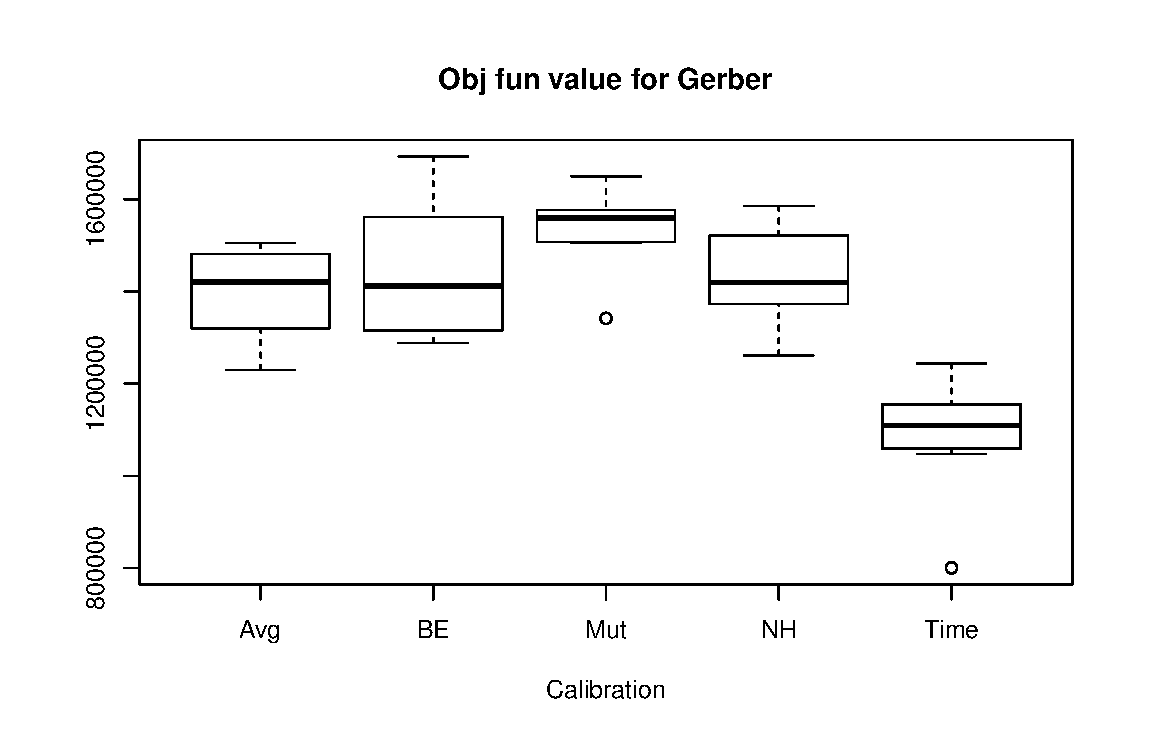
\includegraphics[scale=.4]{pics/boxplots/gerber.eps}}
\end{minipage}%
\begin{minipage}{.5\linewidth}
\centering
\subfloat[]{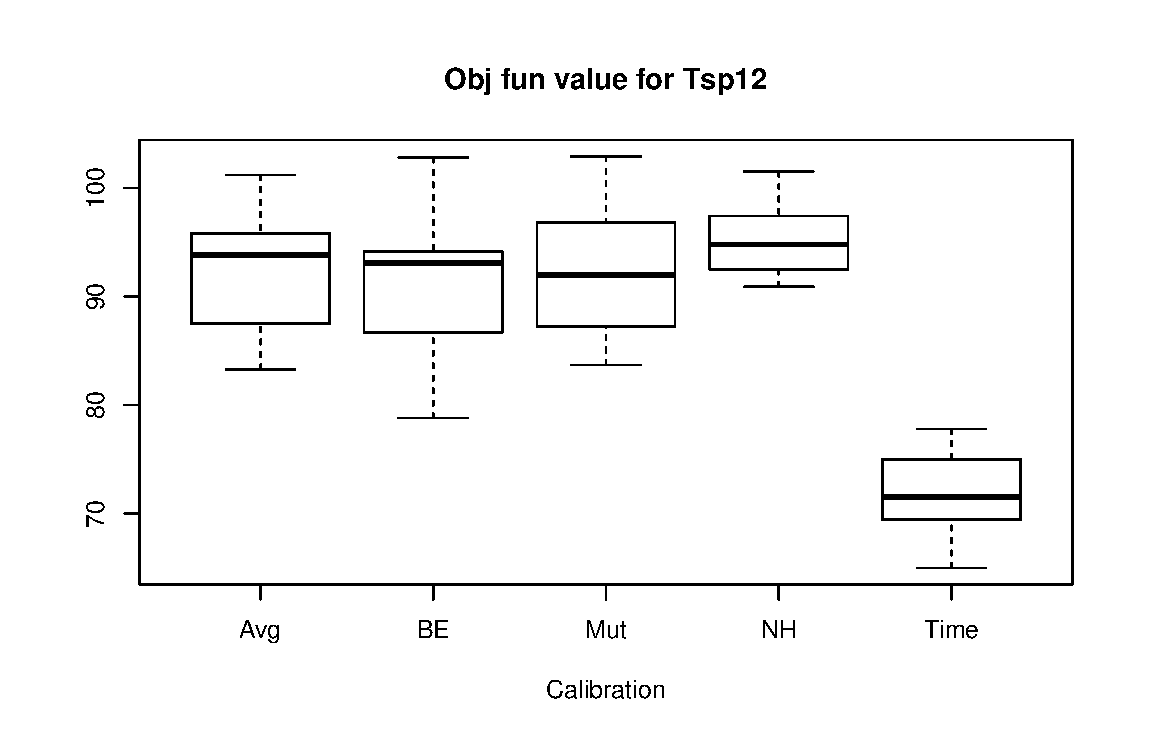
\includegraphics[scale=.4]{pics/boxplots/tsp12.eps}}
\end{minipage}\par\medskip
\centering
\subfloat[]{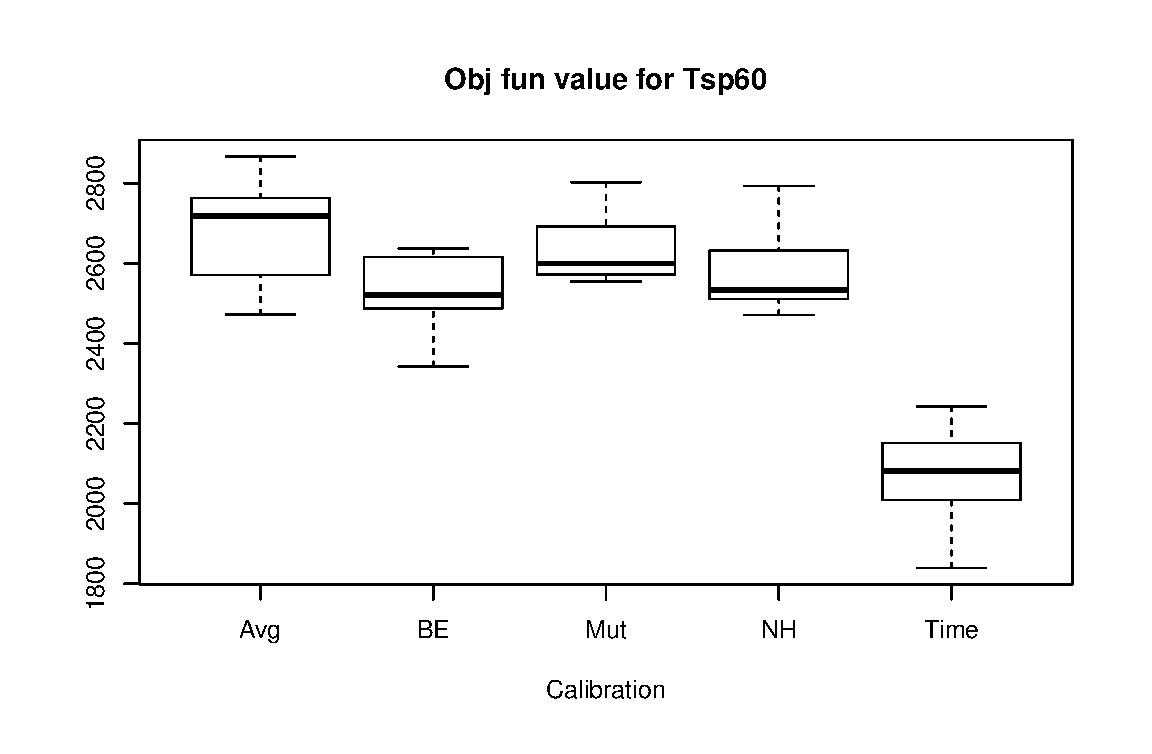
\includegraphics[scale=.4]{pics/boxplots/tsp60.eps}}

\caption{Objective function performance on fixed instances}
\label{fig:obj-fixed}
\end{figure}

%%%%%%%%%%%%%%%%%%%
%% RU 10 holes
%%%%%%%%%%%%%%%%%%%

\begin{figure}[H]

\begin{minipage}{.5\linewidth}
\centering
\subfloat[]{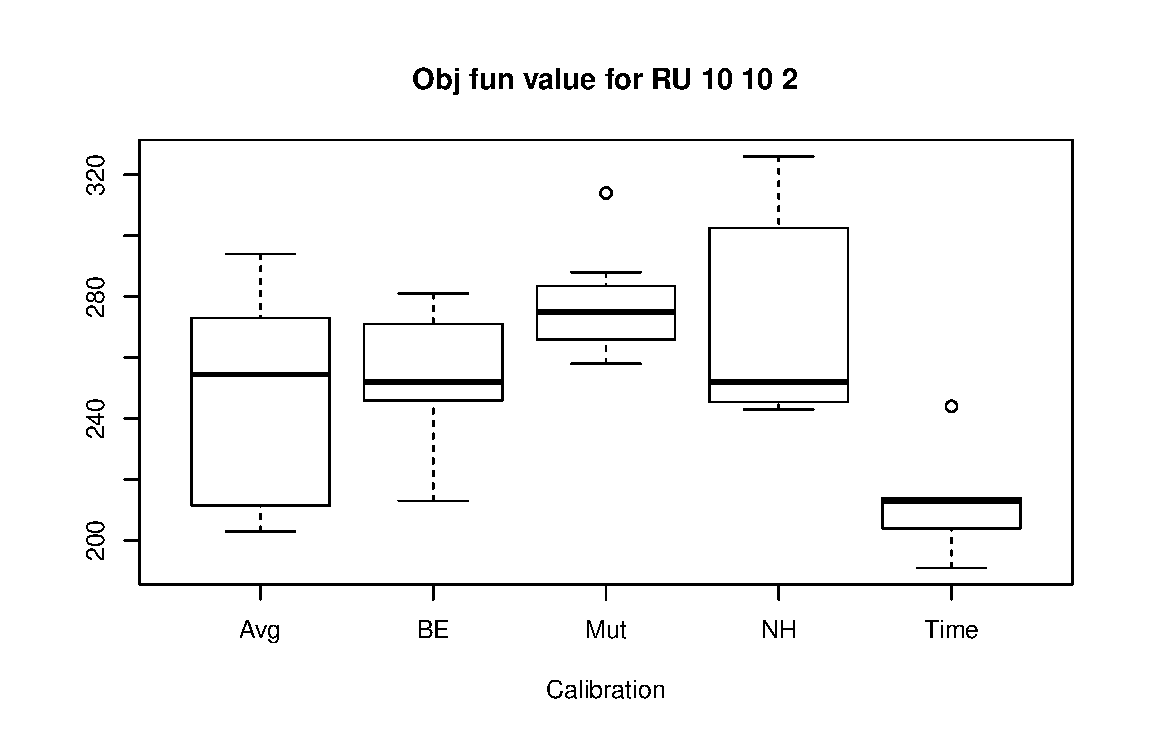
\includegraphics[scale=.4]{pics/boxplots/ru-10-10-2.eps}}
\end{minipage}%
\begin{minipage}{.5\linewidth}
\centering
\subfloat[]{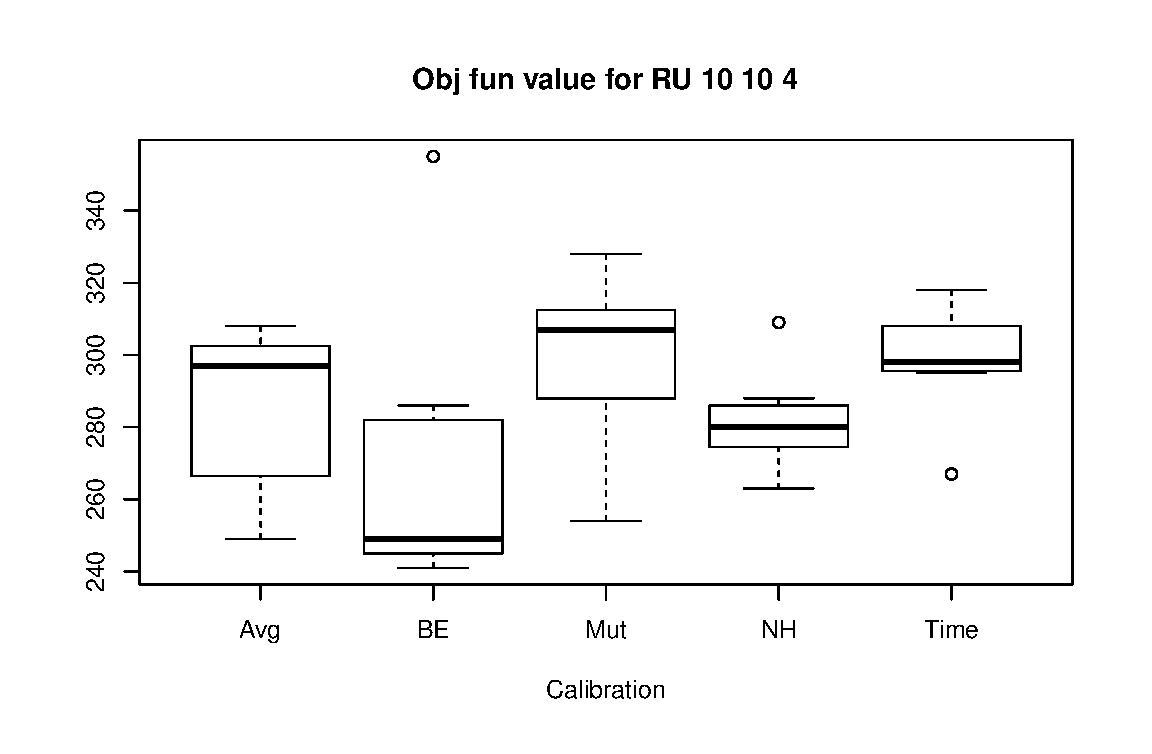
\includegraphics[scale=.4]{pics/boxplots/ru-10-10-4.eps}}
\end{minipage}\par\medskip
\centering
\begin{minipage}{.5\linewidth}
\centering
\subfloat[]{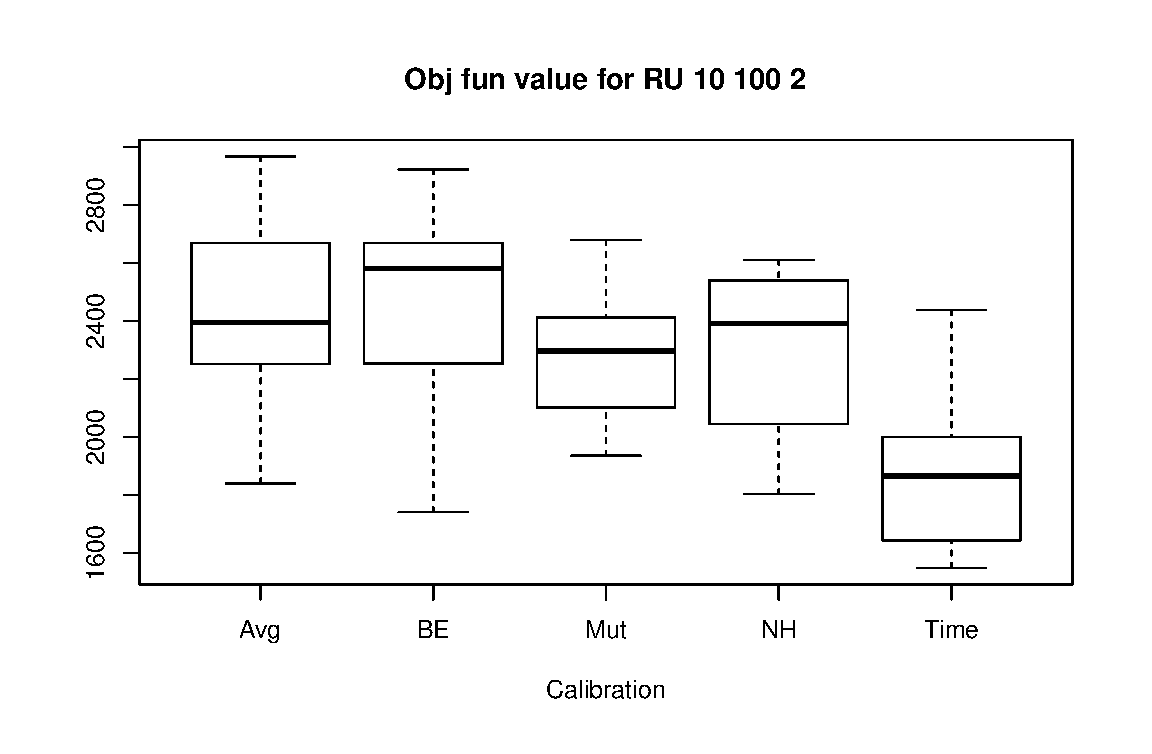
\includegraphics[scale=.4]{pics/boxplots/ru-10-100-2.eps}}
\end{minipage}%
\begin{minipage}{.5\linewidth}
\centering
\subfloat[]{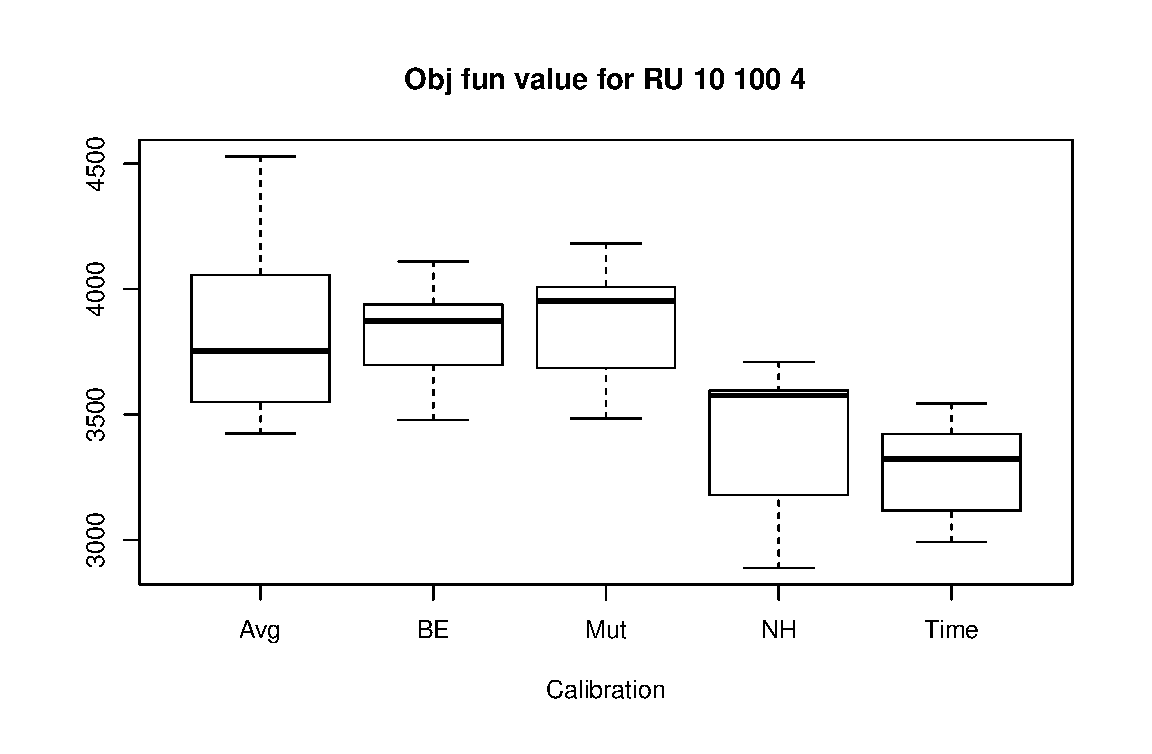
\includegraphics[scale=.4]{pics/boxplots/ru-10-100-4.eps}}
\end{minipage}\par\medskip

\caption{Objective function performance for Random Uniform with 10 holes}
\label{fig:obj-fixed}
\end{figure}

%%%%%%%%%%%%%%%%%%%
%% RU 50 holes
%%%%%%%%%%%%%%%%%%%

\begin{figure}[H]

\begin{minipage}{.5\linewidth}
\centering
\subfloat[]{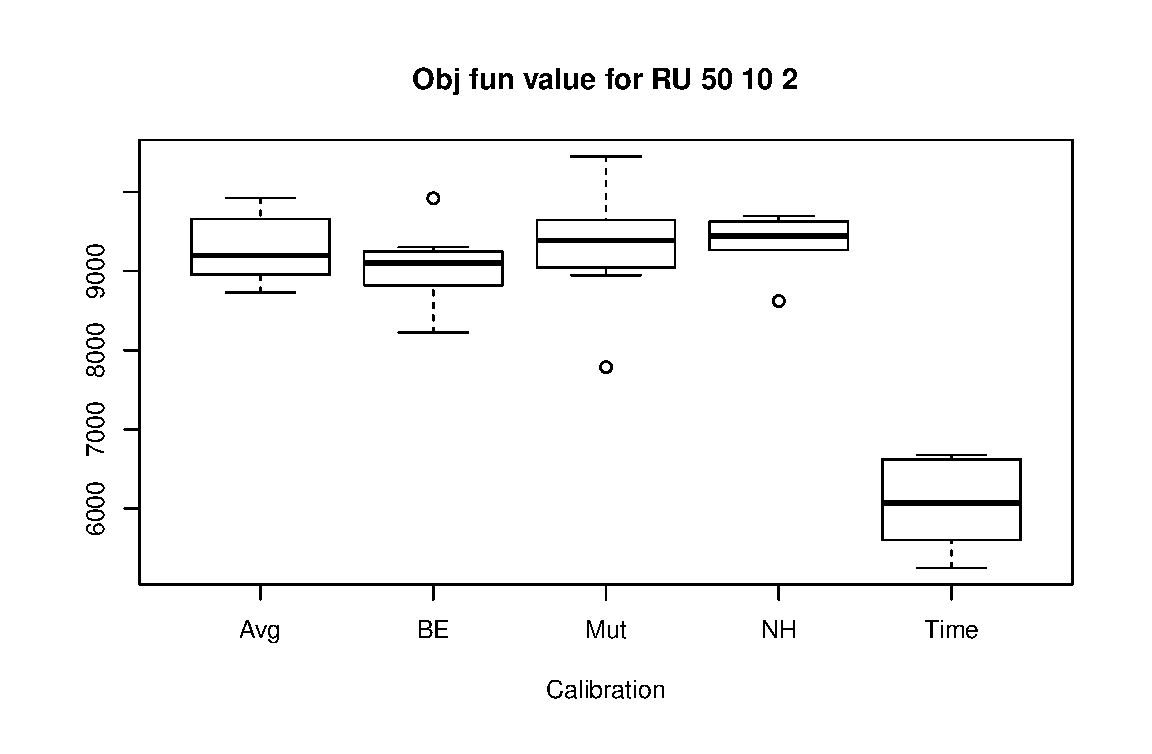
\includegraphics[scale=.4]{pics/boxplots/ru-50-10-2.eps}}
\end{minipage}%
\begin{minipage}{.5\linewidth}
\centering
\subfloat[]{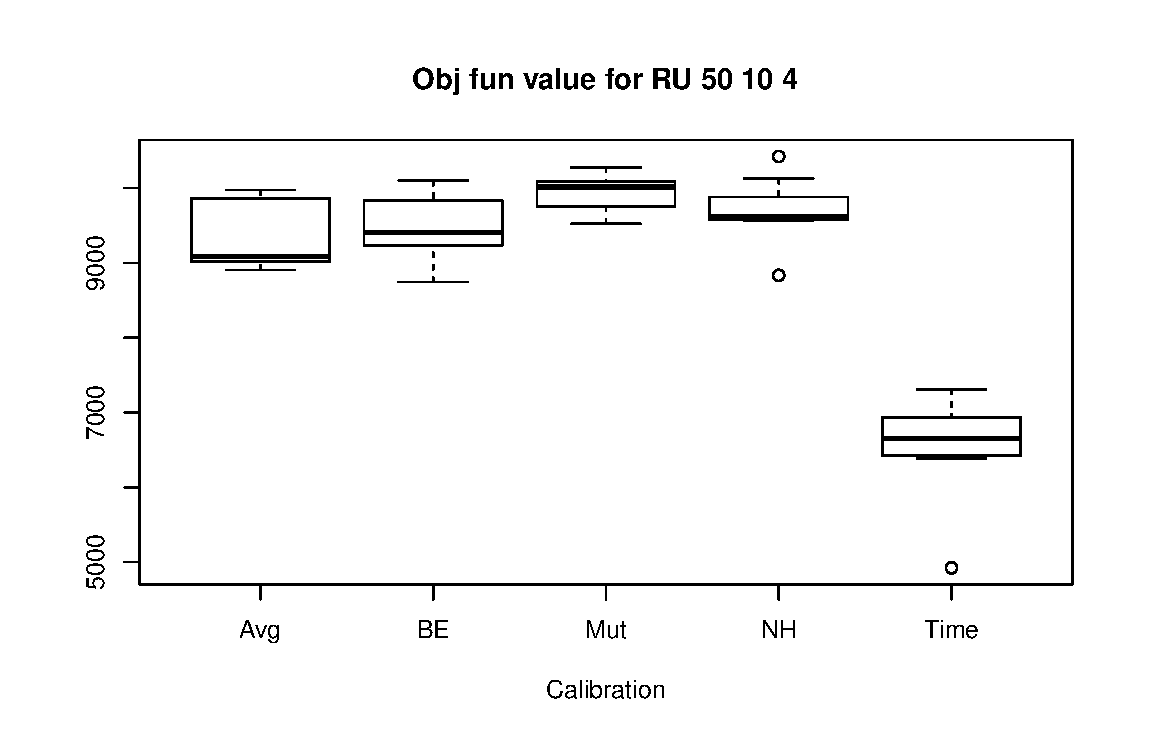
\includegraphics[scale=.4]{pics/boxplots/ru-50-10-4.eps}}
\end{minipage}\par\medskip
\centering
\begin{minipage}{.5\linewidth}
\centering
\subfloat[]{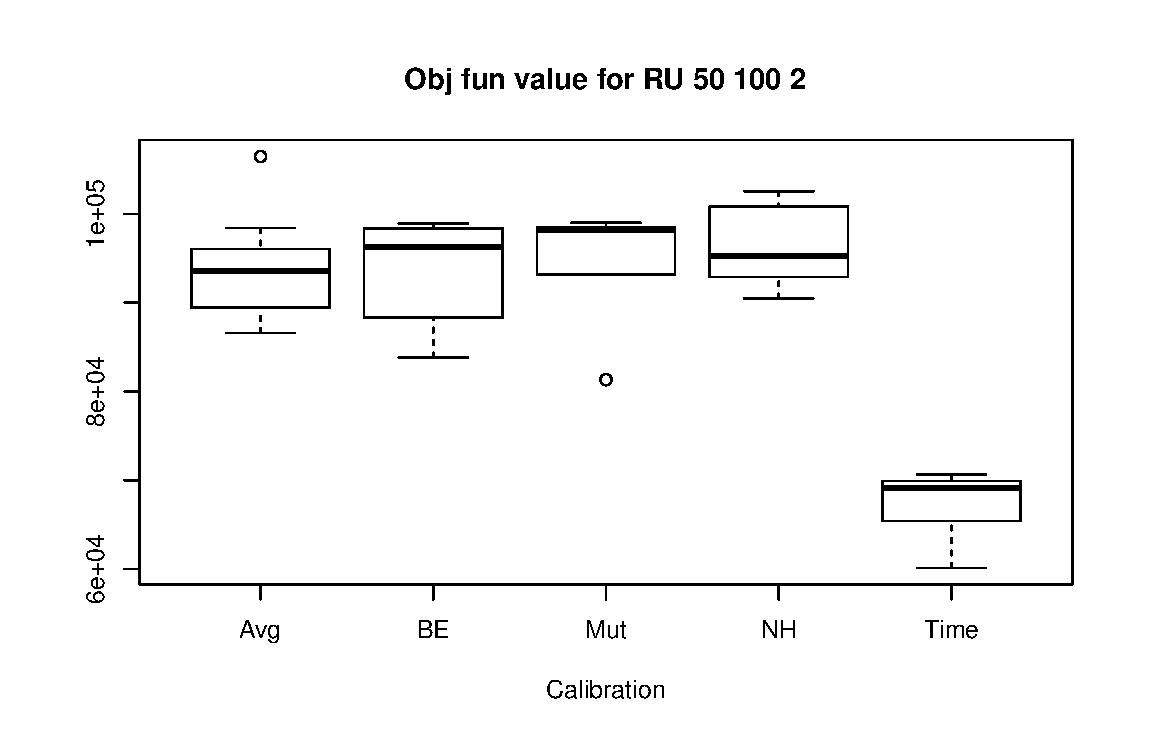
\includegraphics[scale=.4]{pics/boxplots/ru-50-100-2.eps}}
\end{minipage}%
\begin{minipage}{.5\linewidth}
\centering
\subfloat[]{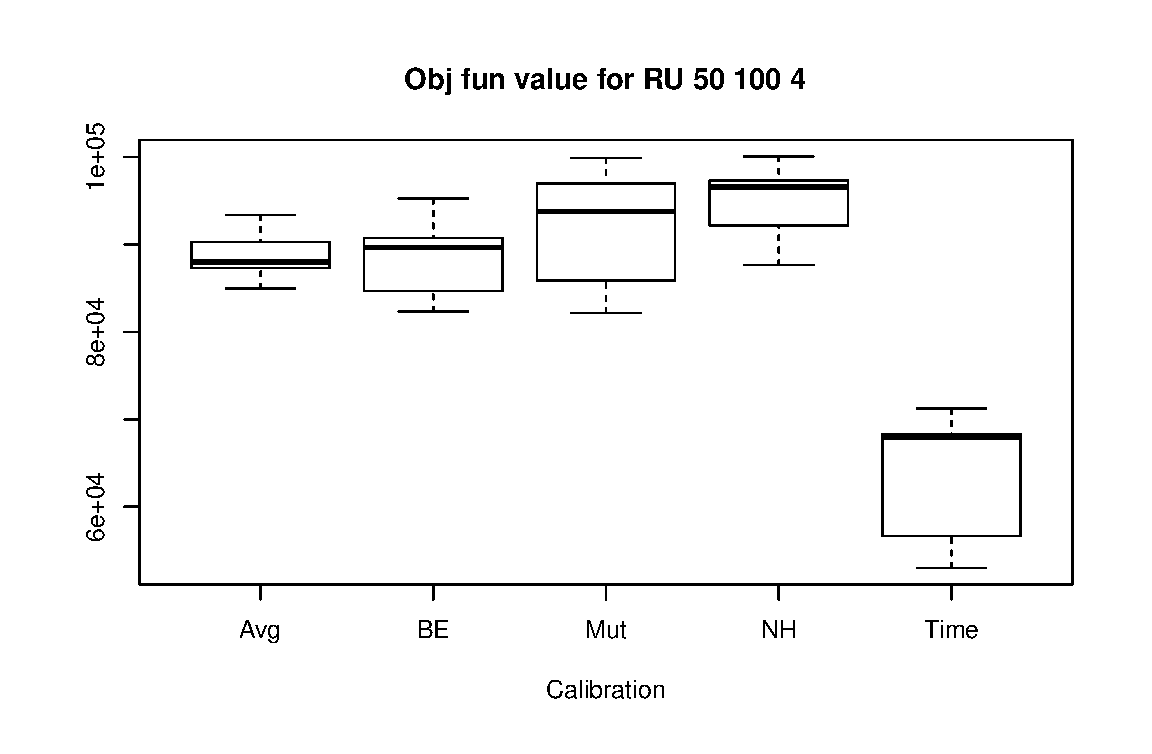
\includegraphics[scale=.4]{pics/boxplots/ru-50-100-4.eps}}
\end{minipage}\par\medskip

\caption{Objective function performance for Random Uniform with 50 holes}
\label{fig:obj-fixed}
\end{figure}

%%%%%%%%%%%%%%%%%%%
%% RG 10 holes
%%%%%%%%%%%%%%%%%%%

\begin{figure}[H]

\begin{minipage}{.5\linewidth}
\centering
\subfloat[]{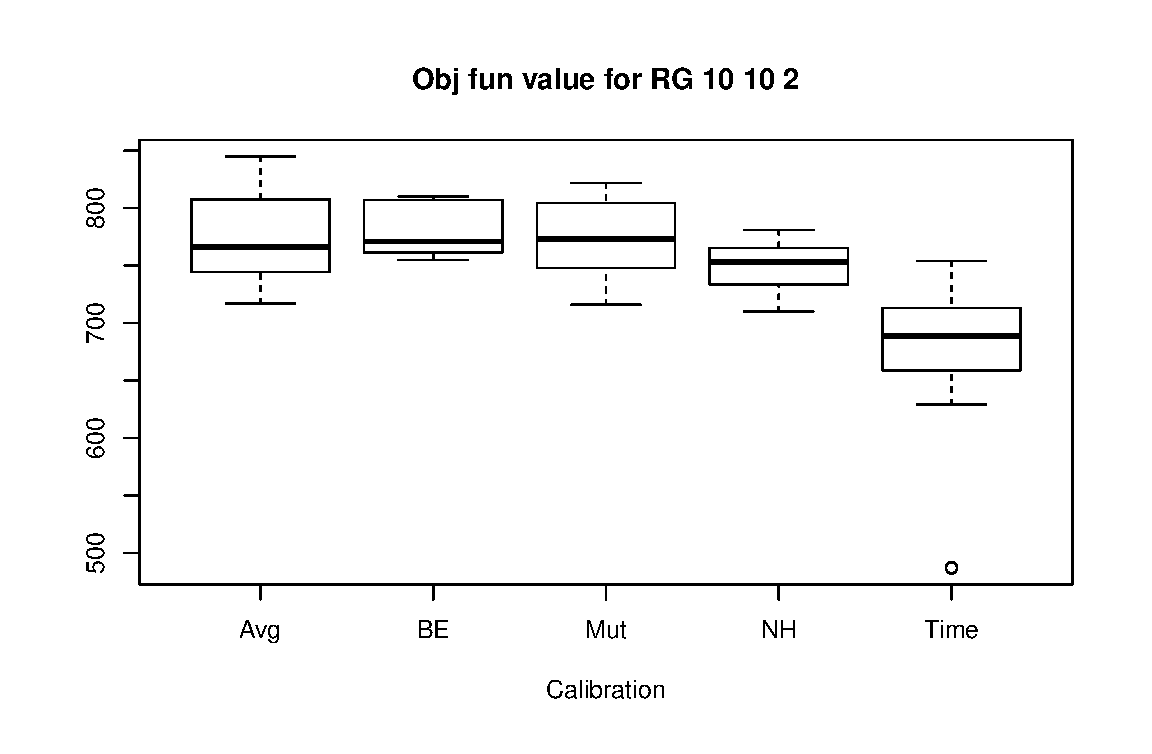
\includegraphics[scale=.4]{pics/boxplots/rg-10-10-2.eps}}
\end{minipage}%
\begin{minipage}{.5\linewidth}
\centering
\subfloat[]{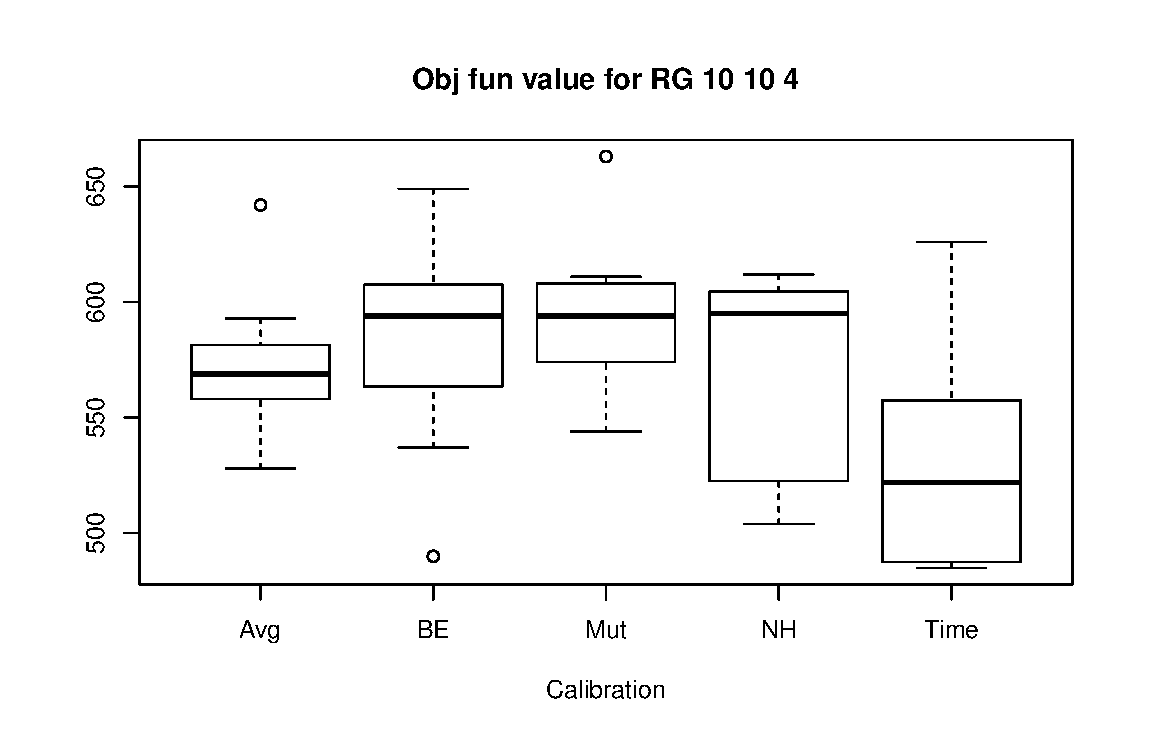
\includegraphics[scale=.4]{pics/boxplots/rg-10-10-4.eps}}
\end{minipage}\par\medskip
\centering
\begin{minipage}{.5\linewidth}
\centering
\subfloat[]{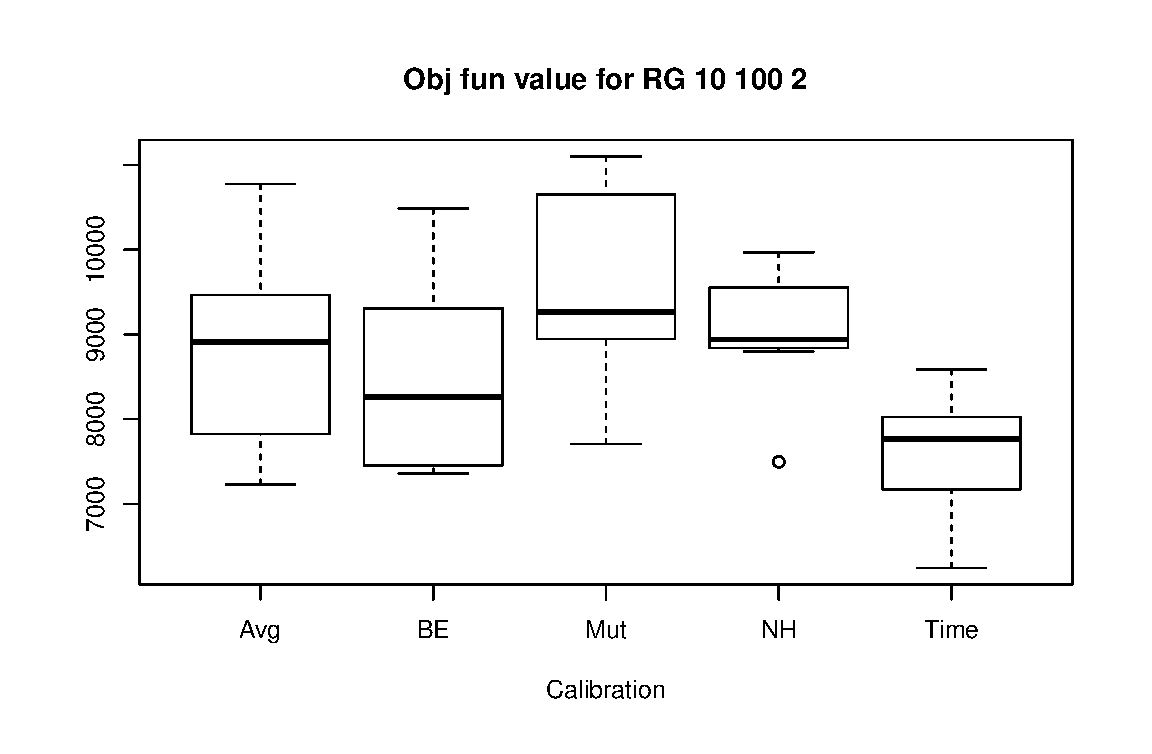
\includegraphics[scale=.4]{pics/boxplots/rg-10-100-2.eps}}
\end{minipage}%
\begin{minipage}{.5\linewidth}
\centering
\subfloat[]{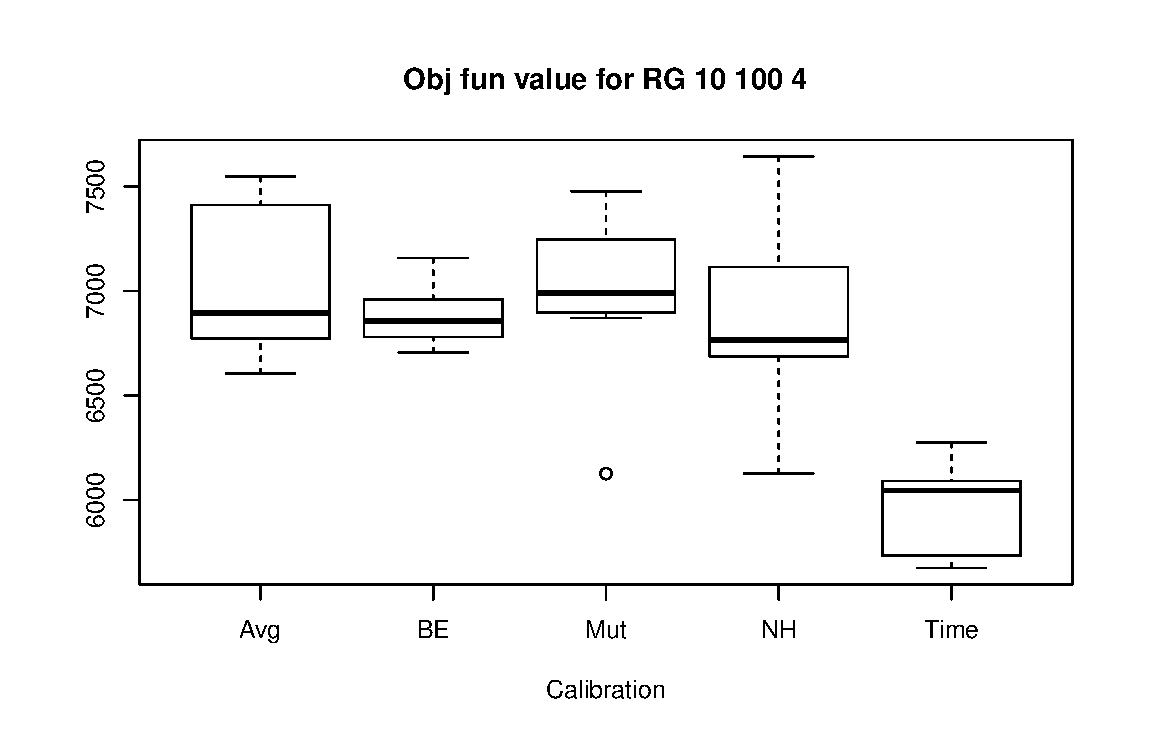
\includegraphics[scale=.4]{pics/boxplots/rg-10-100-4.eps}}
\end{minipage}\par\medskip

\caption{Objective function performance for Random Grid Uniform with 10 holes}
\label{fig:obj-fixed}
\end{figure}


%%%%%%%%%%%%%%%%%%%
%% RG 50 holes
%%%%%%%%%%%%%%%%%%%

\begin{figure}[H]

\begin{minipage}{.5\linewidth}
\centering
\subfloat[]{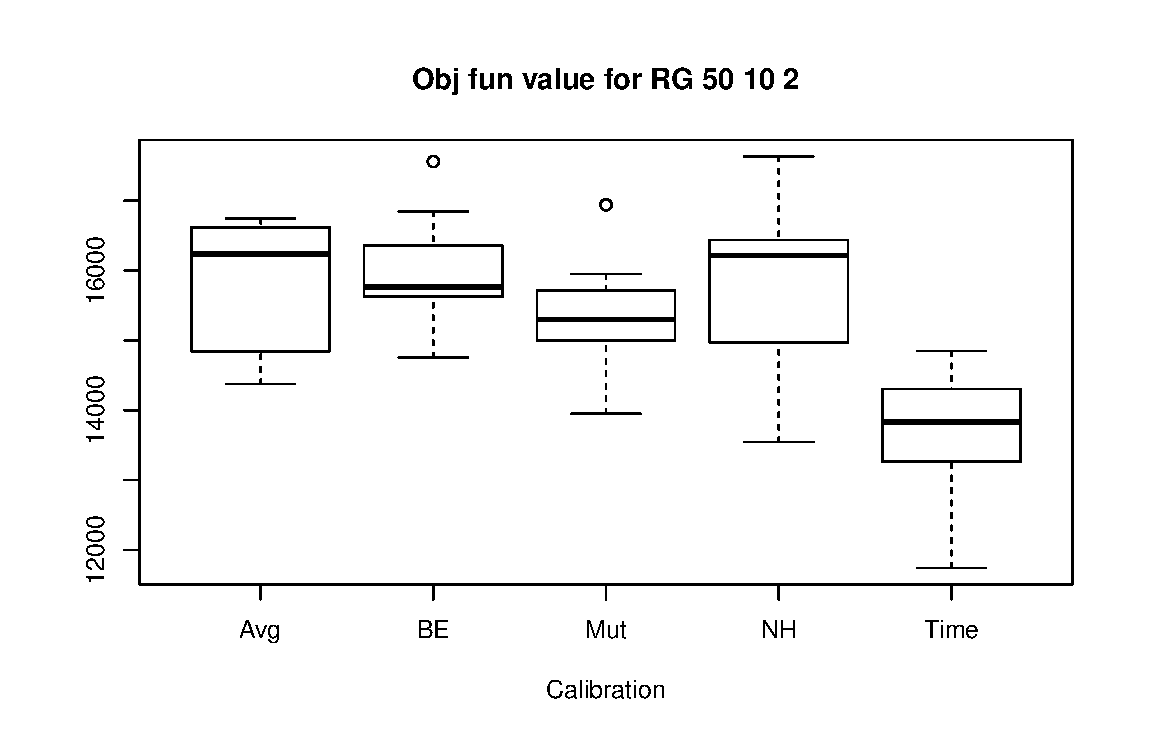
\includegraphics[scale=.4]{pics/boxplots/rg-50-10-2.eps}}
\end{minipage}%
\begin{minipage}{.5\linewidth}
\centering
\subfloat[]{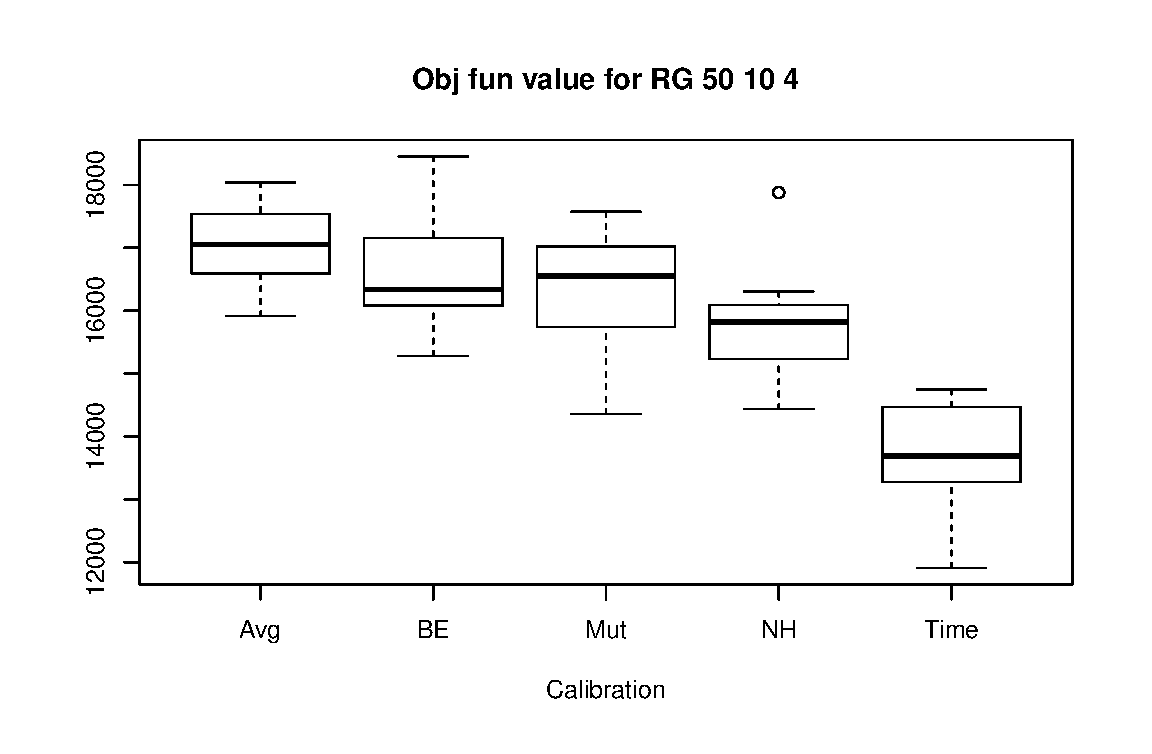
\includegraphics[scale=.4]{pics/boxplots/rg-50-10-4.eps}}
\end{minipage}\par\medskip
\centering
\begin{minipage}{.5\linewidth}
\centering
\subfloat[]{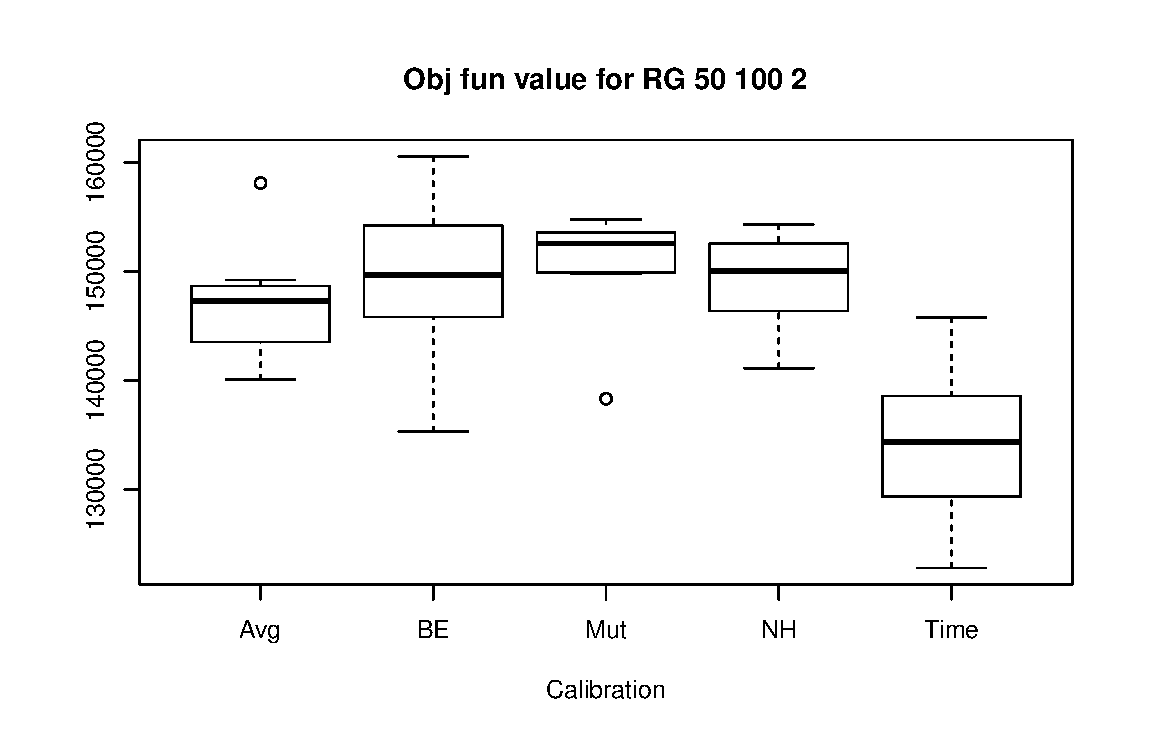
\includegraphics[scale=.4]{pics/boxplots/rg-50-100-2.eps}}
\end{minipage}%
\begin{minipage}{.5\linewidth}
\centering
\subfloat[]{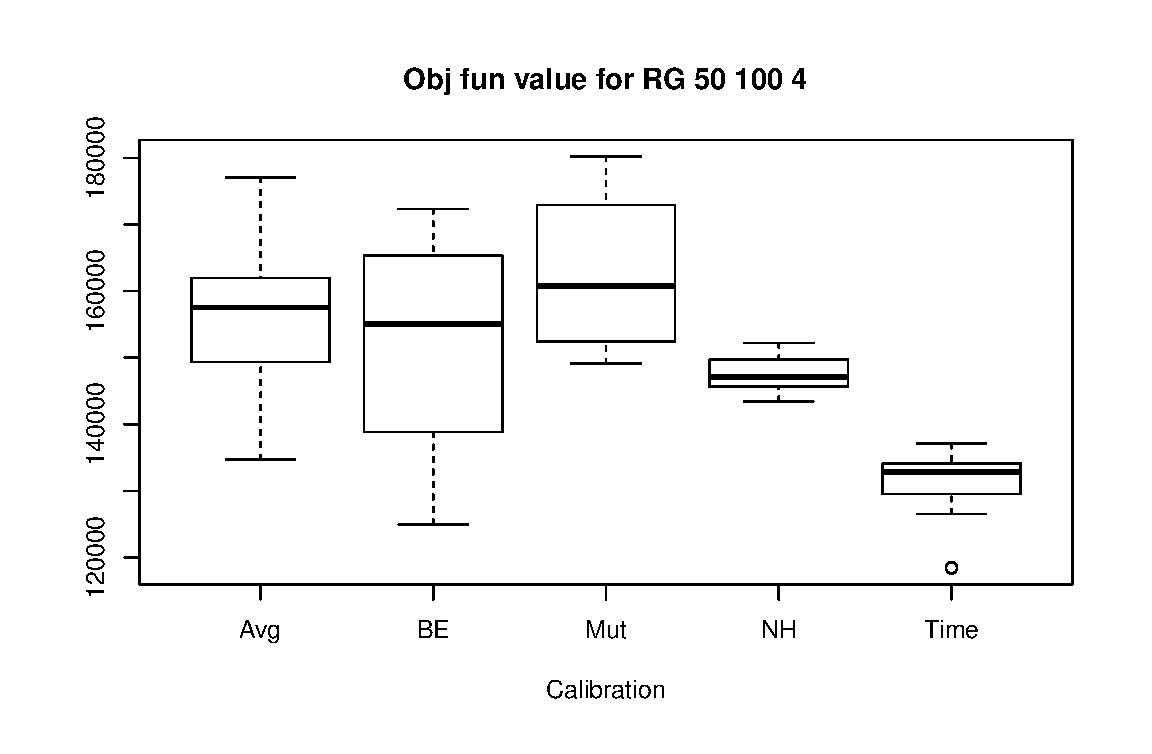
\includegraphics[scale=.4]{pics/boxplots/rg-50-100-4.eps}}
\end{minipage}\par\medskip

\caption{Objective function performance for Random Grid Uniform with 50 holes}
\label{fig:obj-fixed}
\end{figure}


%%%%%%%%%%%%%%%%%%%
%% RG MANH 10 holes
%%%%%%%%%%%%%%%%%%%

\begin{figure}[H]

\begin{minipage}{.5\linewidth}
\centering
\subfloat[]{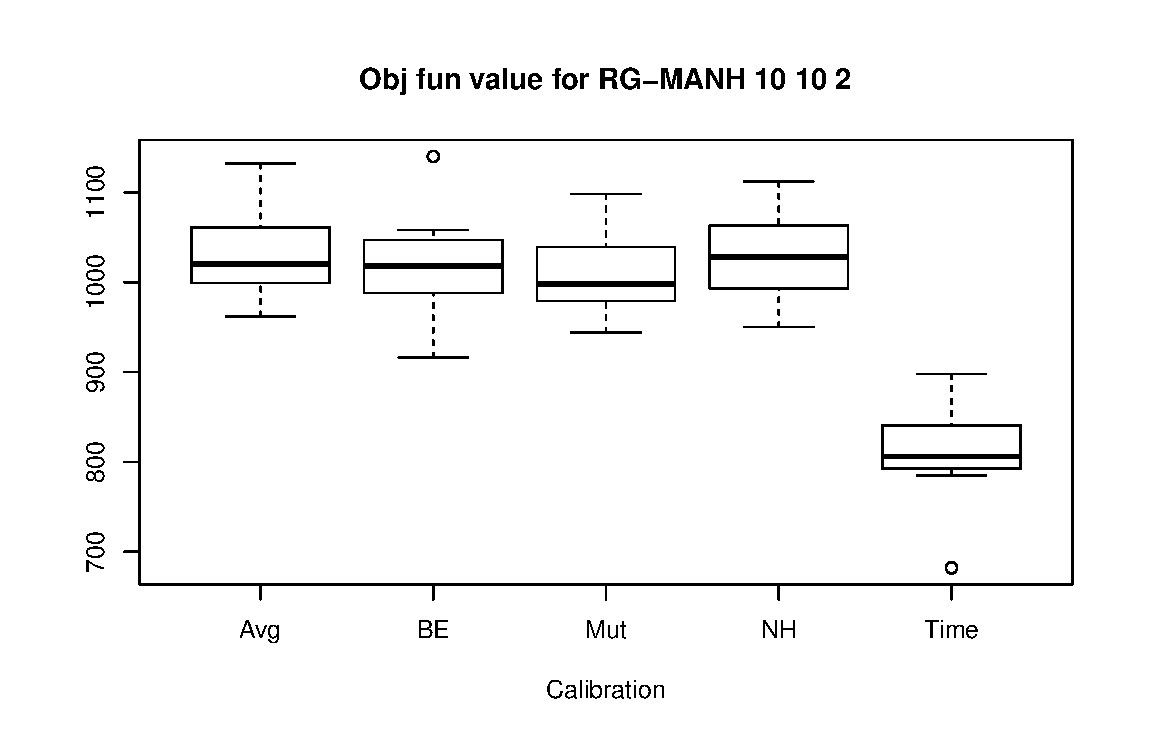
\includegraphics[scale=.4]{pics/boxplots/rg-manh-10-10-2.eps}}
\end{minipage}%
\begin{minipage}{.5\linewidth}
\centering
\subfloat[]{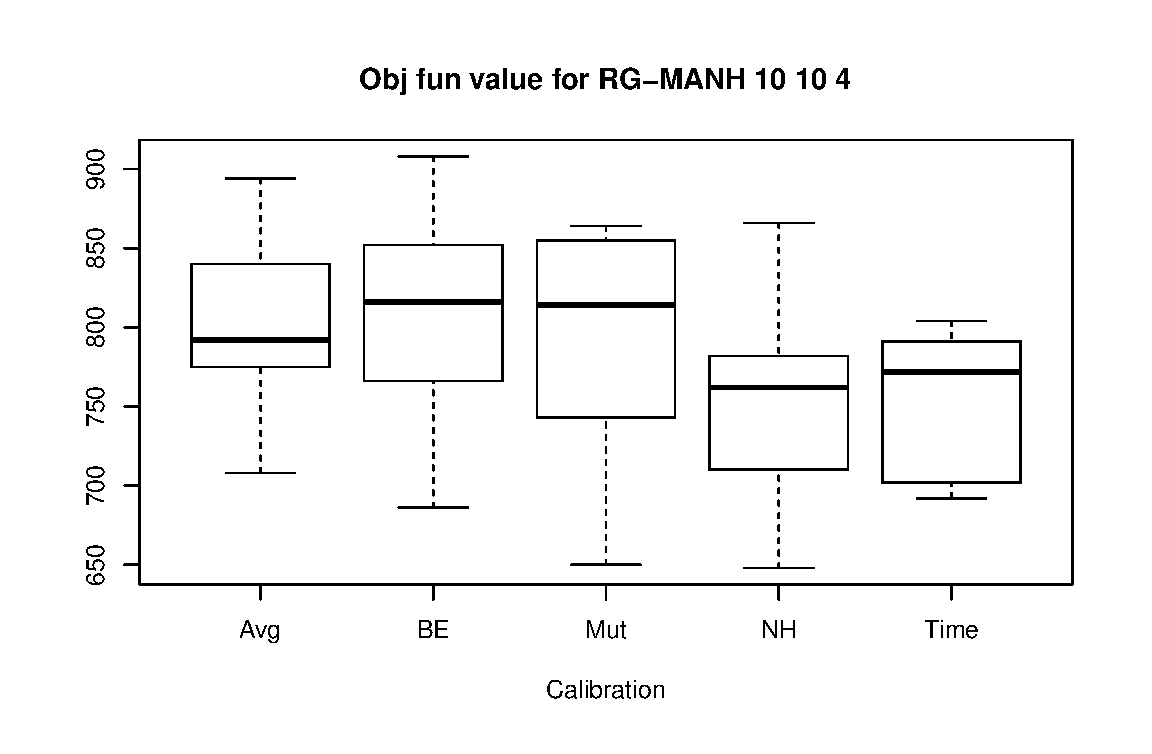
\includegraphics[scale=.4]{pics/boxplots/rg-manh-10-10-4.eps}}
\end{minipage}\par\medskip
\centering
\begin{minipage}{.5\linewidth}
\centering
\subfloat[]{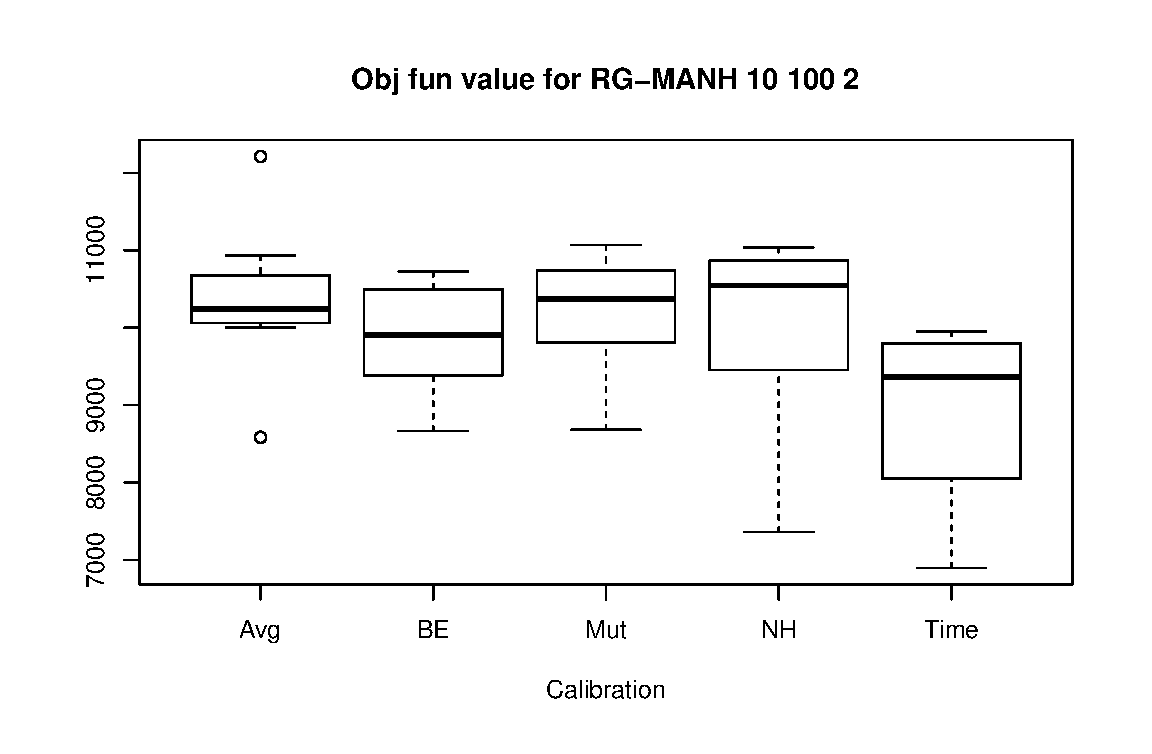
\includegraphics[scale=.4]{pics/boxplots/rg-manh-10-100-2.eps}}
\end{minipage}%
\begin{minipage}{.5\linewidth}
\centering
\subfloat[]{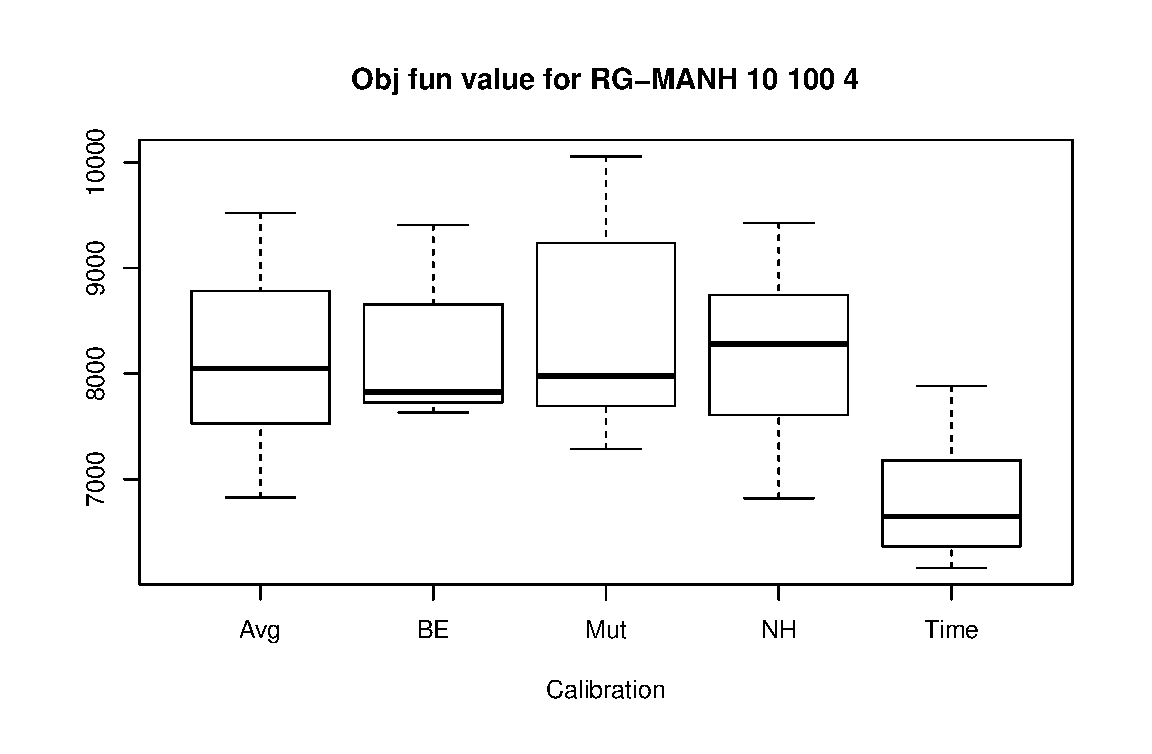
\includegraphics[scale=.4]{pics/boxplots/rg-manh-10-100-4.eps}}
\end{minipage}\par\medskip

\caption{Objective function performance for Random Grid Uniform (Manhattan
  distance) with 10 holes}
\label{fig:obj-fixed}
\end{figure}


%%%%%%%%%%%%%%%%%%%
%% RG MANH 50 holes
%%%%%%%%%%%%%%%%%%%

\begin{figure}[H]

\begin{minipage}{.5\linewidth}
\centering
\subfloat[]{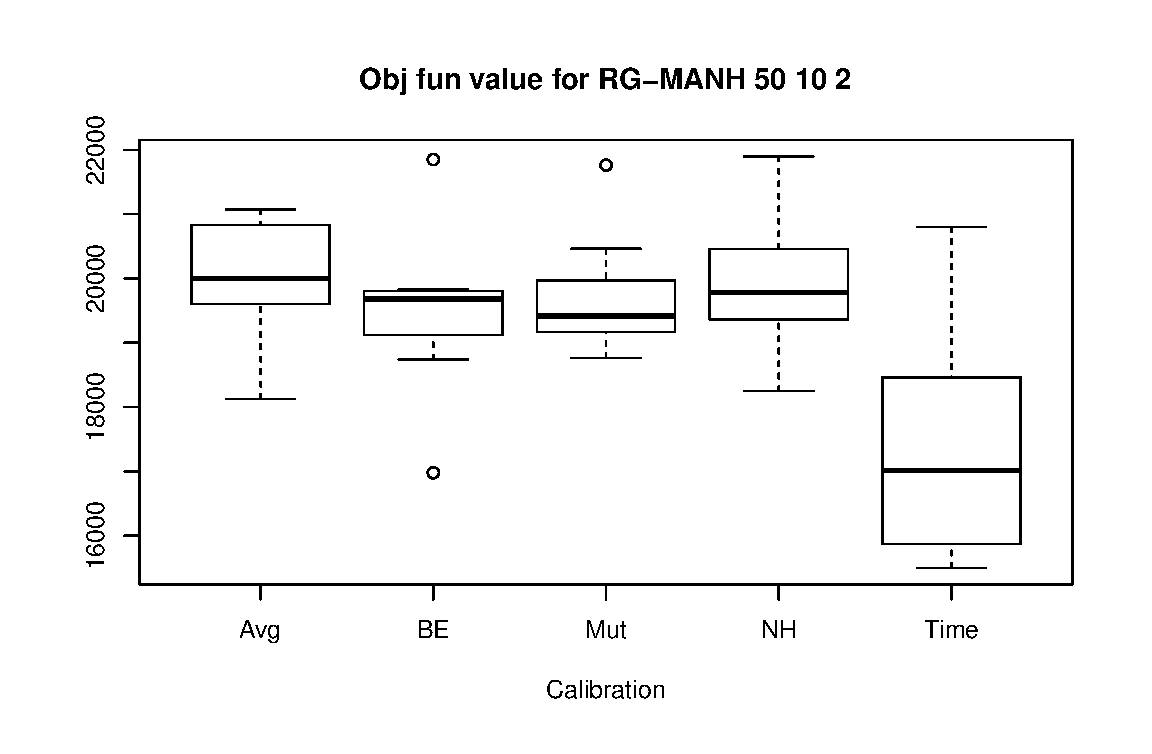
\includegraphics[scale=.4]{pics/boxplots/rg-manh-50-10-2.eps}}
\end{minipage}%
\begin{minipage}{.5\linewidth}
\centering
\subfloat[]{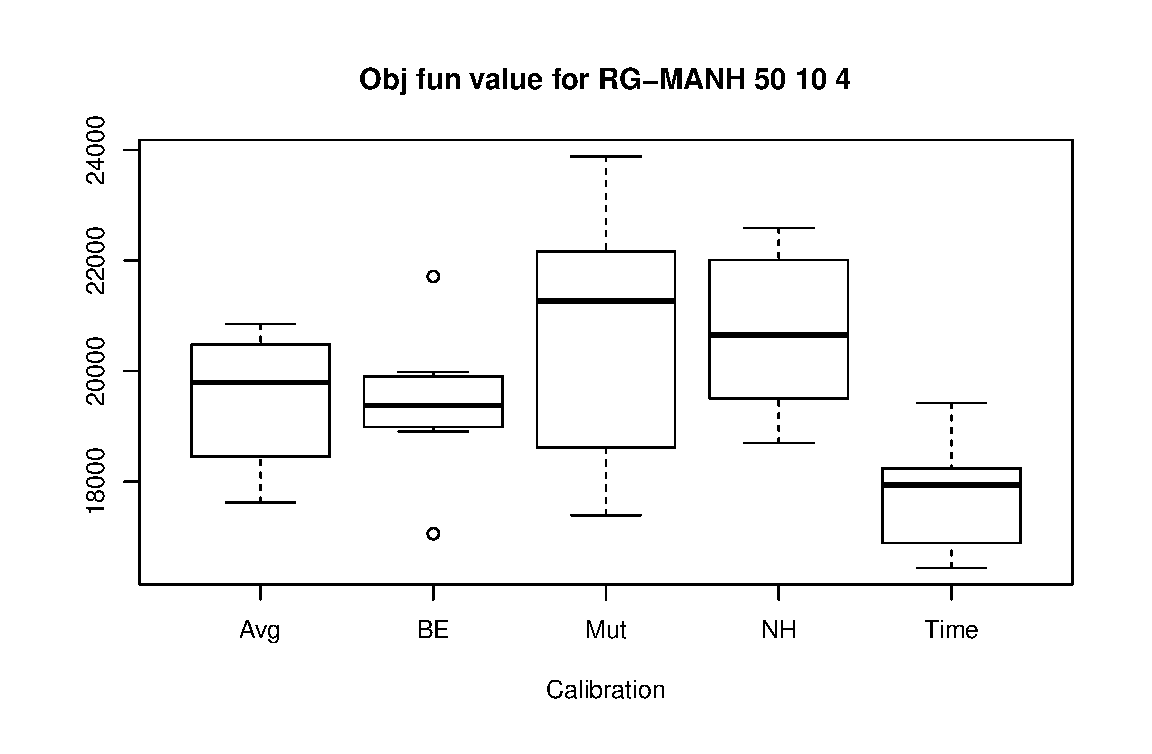
\includegraphics[scale=.4]{pics/boxplots/rg-manh-50-10-4.eps}}
\end{minipage}\par\medskip
\centering
\begin{minipage}{.5\linewidth}
\centering
\subfloat[]{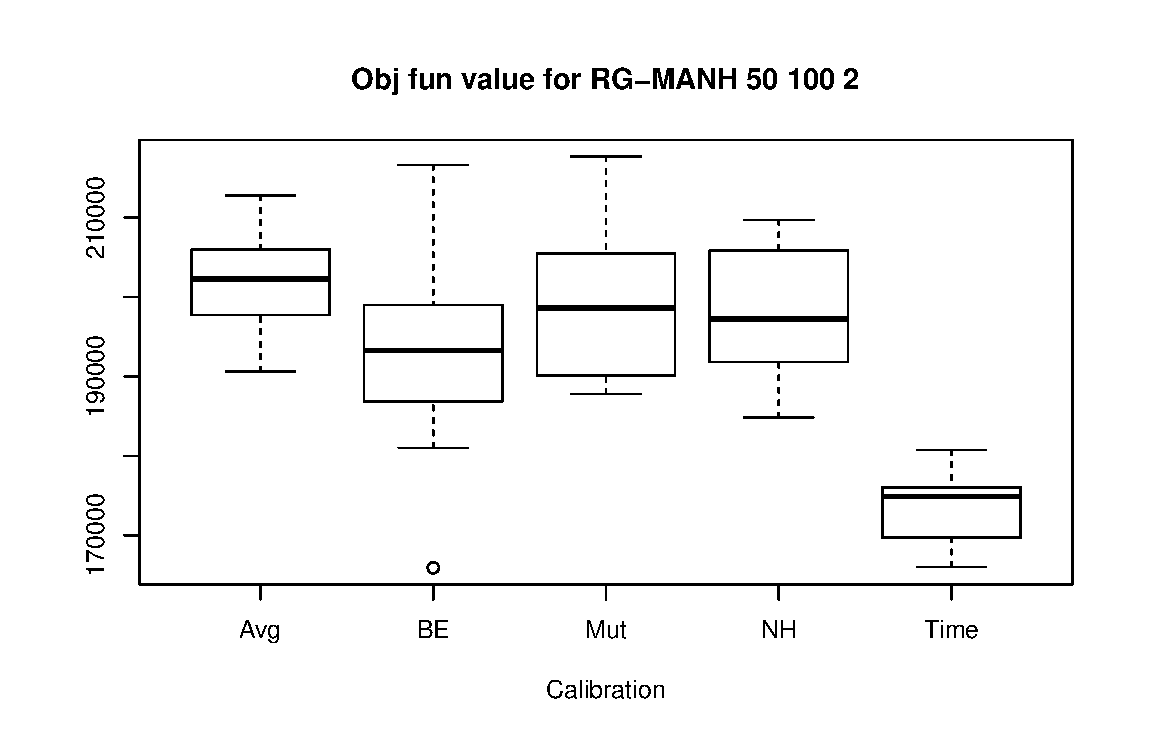
\includegraphics[scale=.4]{pics/boxplots/rg-manh-50-100-2.eps}}
\end{minipage}%
\begin{minipage}{.5\linewidth}
\centering
\subfloat[]{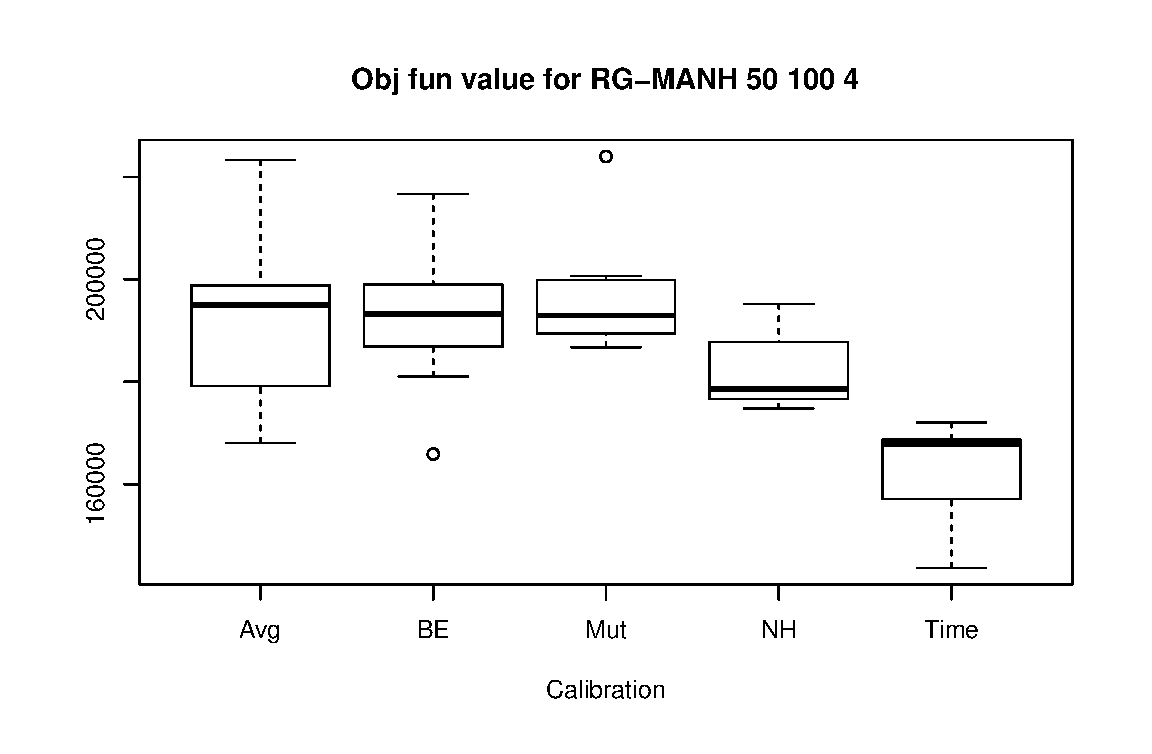
\includegraphics[scale=.4]{pics/boxplots/rg-manh-50-100-4.eps}}
\end{minipage}\par\medskip

\caption{Objective function performance for Random Grid Uniform (Manhattan
  distance) with 50 holes}
\label{fig:obj-fixed}
\end{figure}

We can make some observations on this graphs:

\begin{itemize}
  \item in almost all the graphs, \textbf{Time} tuning yielded the best
    performance in terms of objective function goodness\footnote{but it was 12
    slower in terms of efficiency}, to the point that sometimes the worst
    result achieved with this calibration outscored all the other tunings;
  \item the time component effect was minor in instances which size was pretty
    small (like 10 or 12 holes). In these cases, no method beat the
    others, but an high mutation rate often lead decent scores on randomly
    generated instances;
  \item for a high number of tests, it's true that \textbf{Mut} and
    \textbf{NH} implied a low variance among the different measurings (you can
    see it because they often have the shortest whiskers);
  \item \textbf{Avg} and \textbf{BE} produced very similar values (looking at
    the plots). Thus, I may argue that the elite size is not so significant
    for the genetic algorithm I have developed as long as there is a high
    number of offspring;
  \item it's nice to see that for the more realistic configuration (i.e. the
    Gerber one), both \textbf{Avg} and \textbf{NH} had similar results. So I
    can suppose that for realistic instances having or not an initial
    population generated with Simulated Annealing is not that relevant.
\end{itemize}

As we can see, it clearly emerges from the boxplots that the time component
has a definitely strong impact on the goodness on the solution.

%TODO: Add comparison between Part I and Part II
%TODO: add instructions for use
%TODO: Add conclusions


\end{document}
